\documentclass[12pt]{article}
\usepackage{graphicx} % Required for inserting images
\usepackage{float}
\usepackage{listings}
\usepackage[dvipsnames]{xcolor}
\usepackage{geometry}
\usepackage[UTF8]{ctex}
\usepackage{amsmath}


\title{Pre-lecture Problems for Lecture 2:\\ Linear Programming}
\author{B10705034 Wen-Xin, Xu}
\geometry{a4paper,scale=0.8}
\begin{document}
\maketitle
\begin{enumerate}
    \item ($0$ point) Graphically solve the following LP:
          \begin{align*}
              \text{max }  & 5x_1+3x_2              \\
              \text{s.t. } & x_1+x_2 \leq 16        \\
                           & x_1+4x_2 \leq 20       \\
                           & 2x_1+x_2 \geq 6        \\
                           & x_1 \geq0, x_2 \geq 0.
          \end{align*}
          \textbf{Ans.}
          \begin{figure}[H]
              \centering
              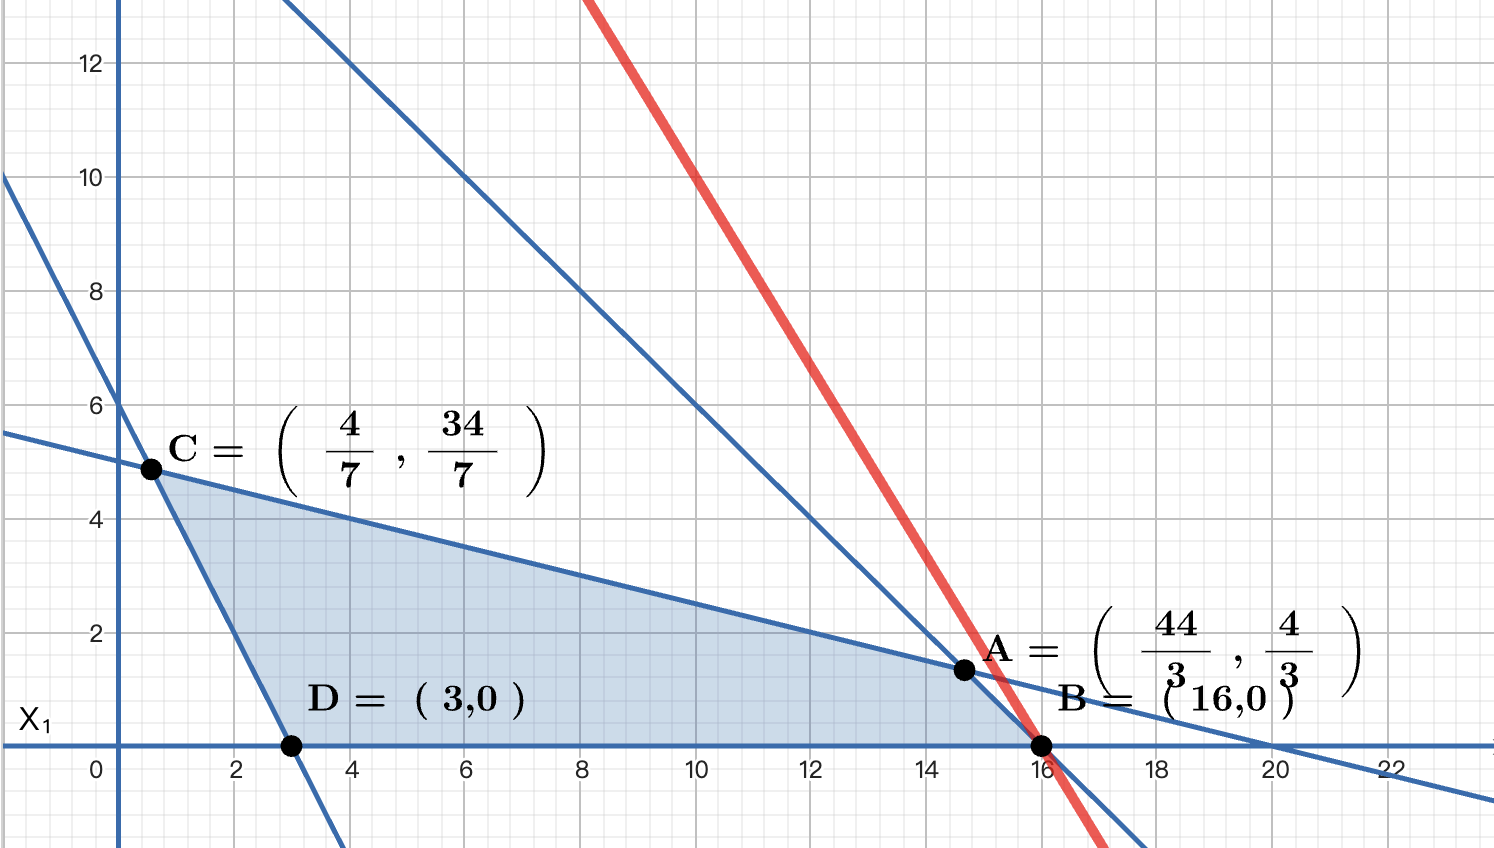
\includegraphics[width=0.5\textwidth]{p1.png}
          \end{figure}
    \item ($0$ point) Bob is the owner of a furniture shop. He uses woods to make tables and chairs. Each day, he buys woods from his supplier at a cost of $\$50$ per unit. Each table requires $2$ units of woods while each chair requires $1$ unit. He, as well as his employees, needs to spend time on making these products. He can make $1$ chair or $0.5$ table in $1$ hour. Each of his two employees, who are not as experiences as him, can make $0.8$ chair or $0.3$ tables in $1$ hour. The outputs are always proportional to the amount of time they spend. Each of the two employees works $8$ hours per day. Bob can work $12$ hours per day. A table can be sold at $200$ and a chair can be sold at $80$. Formulate an LP that can find a production plan for Bob to maximize his daily profit.\\
          \textbf{Ans.}
          We can formulate the LP as follows:\\
          Let $x_1$ be the number of tables and $x_2$ be the number of chairs. Then the LP is
          \begin{align*}
              \text{max }  & 100x_1+30x_2                           \\
              \text{s.t. } & 2x_1+1x_2 \leq 12                      \\
                           & \frac{10}{3}x_1+\frac{5}{4}x_2 \leq 16 \\
                           & x_1 \geq0, x_2 \geq 0.
          \end{align*}
    \item ($10$ points) Tom is the owner of a furniture shop and makes $n$ products. Each day, he buys woods from his supplier at a cost of $C$ dollars per unit. The maximum amount of woods that may be purchased is $K$ units. Each unit of product $j$ requires $Rj$ units of woods, $j = 1, ..., n$. He also needs to spend time on making these products. He can make $Tj$ units of product $j$ per hour, $j = 1, ..., n.$ The outputs are always proportional to the amount of time they spend. Tom can work for $H$ hours per day. Each unit of product $j$ can be sold at $Pj$ dollars. All produced products will be sold.
          \begin{enumerate}
              \item ($5$ points) Formulate an LP that can help make a production plan for Tom to maximize his average daily profit.\\
                    \textbf{Note.} You are required to formulate a "linear program." In particular, there should be no integer constraints on your variables. Therefore, please set your production quantities as fractional variables rather than integer one. If you wonder why $4.7$ tables or $15.2$ chairs are reasonable, you may consider these quantities as the average production quantities per day.\\
                    \textbf{Ans.}
                    We can formulate the LP as follows:\\
                    Let $x_j$ be the number of product $j$. Then the LP is
                    \begin{align*}
                        \text{max }  & \sum_{j=1}^{n} (P_j-C\cdot R_j)x_j \\
                        \text{s.t. } & \sum_{j=1}^{n} R_jx_j \leq K       \\
                                     & \sum_{j=1}^{n} T_jx_j \leq H       \\
                                     & x_j \geq 0, j = 1, ..., n.
                    \end{align*}
              \item ($5$ points) Let $n=2,\ C=15,\ K=300,\ R_1 =8,\ R_2 =5,\ T_1 =3,\ T_2 =4,\ H=10,\ P_1 =100$, and $P_2 = 80$. Graphically solve the LP. Interpret your solution to make a suggestion to Tom.\\
                    \textbf{Ans.}
                    We can formulate the LP as follows:\\
                    Let $x_1$ be the number of product $1$ and $x_2$ be the number of product $2$. Then the LP is
                    \begin{align*}
                        \text{max }  & -20x_1+5x_2             \\
                        \text{s.t. } & 8x_1+5x_2 \leq 300      \\
                                     & 3x_1+4x_2 \leq 10       \\
                                     & x_1 \geq 0, x_2 \geq 0.
                    \end{align*}
                    \begin{figure}[H]
                        \centering
                        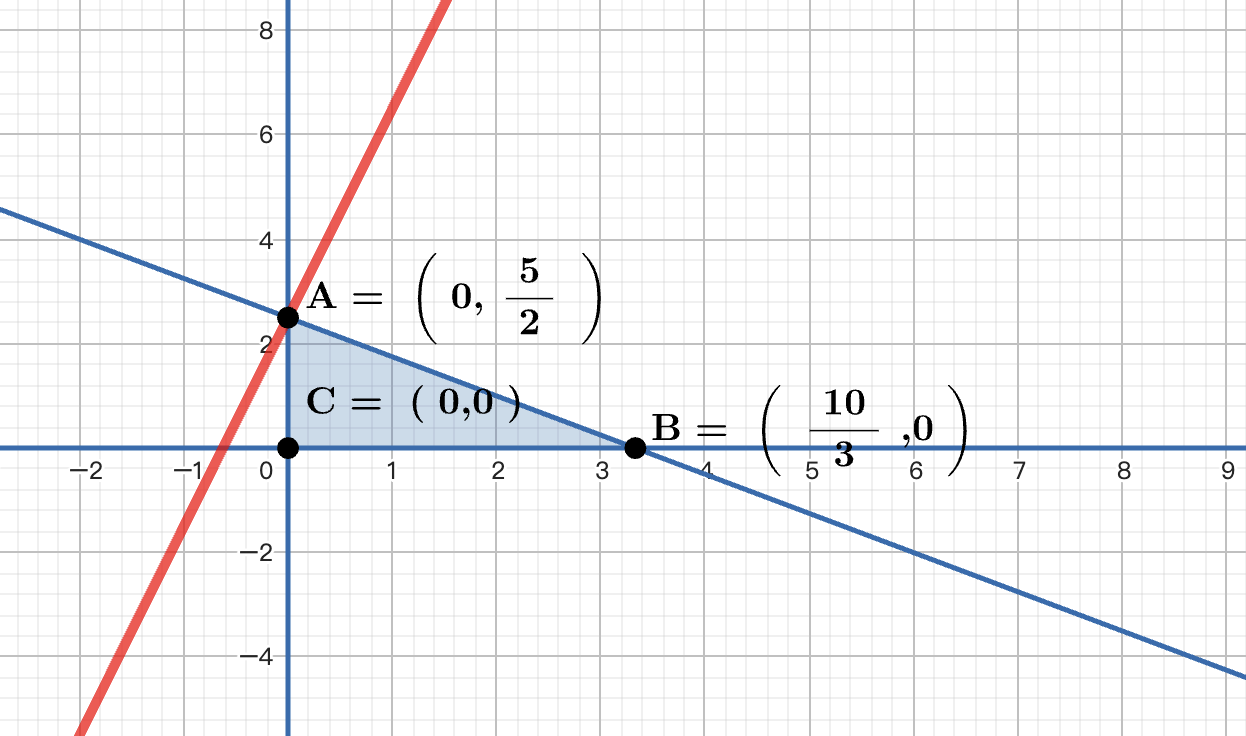
\includegraphics[width=0.5\textwidth]{p3.png}
                    \end{figure}
                    As the graph shows, the optimal solution is $(0, \frac{5}{2})$.
                    I suggest that Tom should spend all his time on product $2$.
          \end{enumerate}
\end{enumerate}
\end{document}

